\begin{frame}{秋にジェットが最も強く、\\対流圏の風向は年中読みやすい}{結果：北海道}
  \begin{columns}[T]
    \begin{column}{0.62\textwidth}
      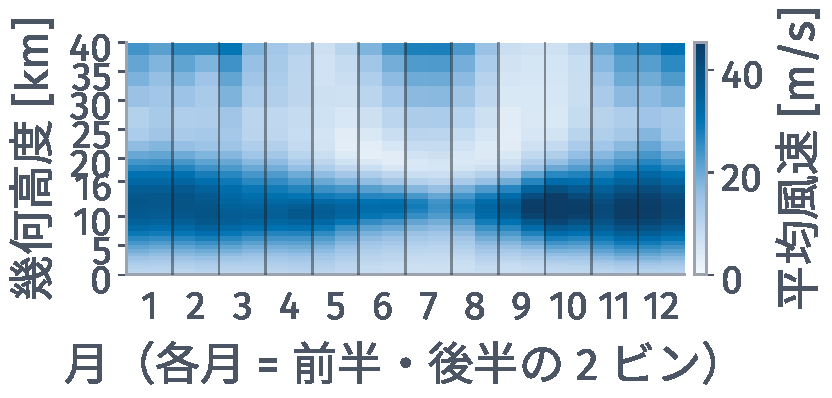
\includegraphics[width=\linewidth,height=96pt,keepaspectratio]{S_alt_half_speed.pdf}
      \vskip 0.5mm
      \sub{ジェットは冬に最強で、同時に南へ下がる。\\北海道には \kw{10--11 月に核が通過}する。}
    \end{column}
    \begin{column}{0.30\textwidth}
      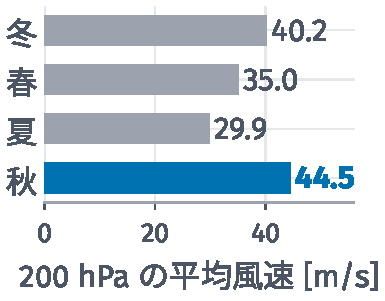
\includegraphics[width=\linewidth,height=88pt,keepaspectratio]{S_season_speed_200.pdf}
      \vskip 0.5mm
      \sub{定常度 \kw{0.81--0.96}、\\風向は年中信用できる。}
    \end{column}
  \end{columns}
  \srcline{北海道 570 格子点の領域平均、2016--2025。和歌山の最強は冬（75.5 m/s）}
\end{frame}
